% LTeX: language=en-GB
%Author(s), Course variables
\newcommand{\titl}{02132 Assignment 2 report}
\newcommand{\subtitl}{Hardware implementation in Chisel\\of a small CPU running the image erosion}
\newcommand{\authone}{Mikkel Arn Andersen}
\newcommand{\SIDone}{s224187}
\newcommand{\authtwo}{Niclas Juul Schæffer}
\newcommand{\SIDtwo}{s224744}
\newcommand{\auththree}{Rasmus Kronborg Finnemann Wiuff}
\newcommand{\SIDthree}{s163977}
\newcommand{\lb}{\\}
%Basics
\documentclass[a4paper, english]{article}
\usepackage[utf8]{inputenc}
\usepackage[T1]{fontenc}
\usepackage[bitstream-charter]{mathdesign}
\usepackage{babel}
\usepackage[moderate, mathspacing=normal]{savetrees}
%Symbols and scientifics
\usepackage{bm}
\usepackage{physics}
\usepackage{mathtools}
\numberwithin{equation}{section}
\usepackage{siunitx}
\sisetup{
per-mode = power ,
round-mode = figures ,
round-precision = 3 ,
exponent-mode = input ,
output-decimal-marker = {.} ,
exponent-product = 	imes ,
uncertainty-mode = separate ,
range-phrase = - ,
range-units =  single ,
inter-unit-product = \ensuremath{{\cdot{}}} ,
quantity-product = \ ,
separate-uncertainty-units = single ,
}

%Appendix, TOC and Bibliography
\usepackage{appendix}
\renewcommand\appendixtocname{Appendix}
\usepackage[nottoc]{tocbibind}
\setcounter{tocdepth}{2}
\usepackage{lastpage}

%Figures
\usepackage[svgnames]{xcolor} % Required to specify font color
\usepackage{float}
\usepackage{graphicx}
\usepackage{subcaption}
\usepackage[format=plain,
    labelfont={bf,it,footnotesize},
    textfont={it,footnotesize}]{caption}
% \captionsetup[table]{name=Huskeord}
\captionsetup{font={stretch=0.9}}
\usepackage{wrapfig}
\usepackage[a4paper, centering, rmargin=2.5cm, tmargin=2.5cm, lmargin=2.5cm, bmargin=3.5cm]{geometry}
\usepackage{verbatim}
\usepackage[space]{grffile}
\usepackage[final]{pdfpages}
\usepackage{pdflscape}
\usepackage{multirow}
\usepackage{fontawesome}
\usepackage{tikz}
% \usetikzlibrary{external}
% \tikzexternalize[prefix=tikz/]
\usepackage{circuitikz}
\ctikzset{logic ports = ieee}
\usetikzlibrary{positioning}
\newcommand{\pin}[3]{\node[blue, font = \small, #2] at (#1) {#3};
                     \coordinate (#3) at (#1);}
\newcommand{\port}[4]{\node[circ, #2] (#1) {};
                     \node[#3] at (#1) {#4};}
%Header footer
\usepackage{fancyhdr}
\pagestyle{fancy}
\lhead{02132 Computer Systems \lb Assignment 1 \lb November \nth{12}}
\chead{
\includegraphics[width=.05\textwidth]{DTU}}
\rhead{\authone \ \textbf{\SIDone} \lb \authtwo \ \textbf{\SIDtwo} \lb \auththree \ \textbf{\SIDthree}}
\cfoot{Page \thepage\, of\, \pageref*{LastPage}}
\renewcommand{\headrulewidth}{0.4pt}
\renewcommand{\footrulewidth}{0.4pt}
\setlength{\headheight}{36.75034pt}

%Text tools
\usepackage{listings}
\usepackage{parcolumns}
\usepackage[super]{nth}
\usepackage[normalem]{ulem}
\usepackage{import}
\usepackage{url}
\usepackage{lipsum}
\usepackage{microtype}
\usepackage[pdfencoding=auto, psdextra]{hyperref}
\hypersetup{
    colorlinks   = true, %Colours links instead of ugly boxes
    urlcolor     = blue, %Colour for external hyperlinks
    linkcolor    = blue, %Colour of internal links
    citecolor   = red %Colour of citations
}
\usepackage[capitalise]{cleveref}
% \crefname{table}{Huskeord}{Huskeord}
\usepackage{enumitem}
\newlist{arrowlist}{itemize}{1}
\setlist[arrowlist]{label={\(\rightarrow\)}}
\usepackage{tabularray}
\UseTblrLibrary{booktabs}
\usepackage{todonotes}
\usepackage[square, longnamesfirst, numbers]{natbib}
\usepackage{empheq}
% \usepackage[newfloat, outputdir=/]{minted} % Overleaf minted buildpath fix
\usepackage[newfloat]{minted}
\setminted{fontsize=\small,
           linenos=true}
\usemintedstyle{tango}
\SetupFloatingEnvironment{listing}{listname=Listings}
\captionsetup[listing]{position=top, skip=-1pt}
\newcommand{\im}[3]{\inputminted[linenos=true, python3=true, firstline=#2, lastline=#3]{python}{#1}}
\newcommand{\java}[3]{\inputminted[linenos=true, firstline=#2, lastline=#3]{java}{#1}}
\usepackage{dirtree}

%Definitions and new commands
\newcommand{\degr}{^{\circ}}
\newcommand{\me}{\mathrm{e}}

%Title and sectioning
\def\Vhrulefill{\leavevmode\leaders\hrule height 0.7ex depth \dimexpr0.4pt-0.7ex\hfill\kern0pt}
\usepackage{titlesec}
\usepackage{titling}
\definecolor{DTUred}{cmyk}{0, .91, .72, .23}
\definecolor{FMNgrey}{cmyk}{.73,.43,.53,.38}
%Use letters insted of numbers in section numbering
% \renewcommand{\thesection}{\Alph{section}}
% \renewcommand{\thesubsection}{\Alph{subsection}}

\makeatletter
\newcommand{\github}[1]{%
   \href{#1}{\color{DTUred}\faGithub}%
}
\makeatother

%Algorithms and pseudocode
\newcounter{nalg}[section] % defines algorithm counter for chapter-level
\renewcommand{\thenalg}{\thesection .\arabic{nalg}} %defines appearance of the algorithm counter
\DeclareCaptionLabelFormat{algocaption}{Algoritme \thenalg} % defines a new caption label as Algorithm x.y

\lstnewenvironment{algorithm}[1][] %defines the algorithm listing environment
{
    \refstepcounter{nalg} %increments algorithm number
    \captionsetup{labelformat=algocaption,labelsep=colon} %defines the caption setup for: it ises label format as the declared caption label above and makes label and caption text to be separated by a ':'
    \lstset{ %this is the stype
        mathescape=true,
        frame=tB,
        numbers=left,
        numberstyle=\tiny,
        basicstyle=\scriptsize,
        keywordstyle=\color{black}\bfseries\em,
        keywords={,input, output, return, datatype, function, in, if, else, foreach, for, while, begin, end, do,} %add the keywords you want, or load a language as Rubens explains in his comment above.
        numbers=left,
        xleftmargin=.04\textwidth,
        columns=fullflexible,
        escapechar=\&,
        #1 % this is to add specific settings to an usage of this environment (for instnce, the caption and referable label)
    }
}
{}
\newcommand*{\runtimeAnalysis}[3]{\hfill\makebox[#3em][l]{\(#1\)}\hspace{5em}\makebox[#3em][l]{\(#2\)}}%

\begin{document}

\titleformat{\section}[block]
{\normalfont\Large\scshape\filright\color{DTUred}}{\fbox{\thesection}}{1em}{}

\titleformat{\subsection}
{\titlerule
    \vspace{.8ex}%
    \normalfont\scshape\color{FMNgrey}}
{\thesubsection.}{.5em}{}

\titleformat{\subsubsection}[wrap]
{\normalfont\fontseries{b}\selectfont\filright}
{\thesubsubsection.}{.5em}{}
\titlespacing{\subsubsection}
{12pc}{1.5ex plus .1ex minus .2ex}{1pc}

\title{\vspace{-40mm}\Huge\scshape\color{DTUred} \titl\lb\vspace{-4mm}\rule{4cm}{0.5mm}\lb\Large{\subtitl}}
\date{November \nth{12}}
\preauthor{\begin{center}
        \large \lineskip 0.5em%
        \begin{tabular}[t]{r}}
            \author{\textbf{Group: 22} \lb \lb \authone \ \textbf{\SIDone} \lb \authtwo \ \textbf{\SIDtwo} \lb \auththree \ \textbf{\SIDthree} \lb \href{https://github.com/rwiuff/02132Assignment2}{\color{DTUred}github.com/rwiuff/02132Assignment2} \github{https://github.com/rwiuff/02132Assignment2}}
            \postauthor{\end{tabular}\par\end{center}}
\maketitle

\pagenumbering{arabic}

\thispagestyle{empty}

\section{Work distribution}
\cref{tbl:ansvar} shows the work distribution in the group for this project.
\begin{table}[H]
    \centering
    \caption{Work distribution on the project}\label{tbl:ansvar}
    \begin{tabular}{lll}
        \toprule
        Name                 & Development tasks & Report tasks   \\
        \midrule
        Mikkel Arn Andersen  &                   &                \\
        Niclas Juul Schæffer &                   &                \\
        Rasmus Wiuff         & ISA               & \cref{sec:isa} \\
        \bottomrule
    \end{tabular}
\end{table}
\section{Design}
% \emph{Explain here what the design process was. List and describe your ISA and how the instructions are encoded. List and describe your compiled program (put a reference to attached file if the compiled program is too long to fit here). Show and describe the block diagram of your CPU. Motivate the design decision you made.}
\subsection{ISA and encoding}\label{sec:isa}
The ISA instructions are inspired from Appendix A in the assignment description. Chosen instructions are listed in \cref{tbl:ISA}.
\begin{table}[H]
    \centering
    \caption{Instruction-set architecture used in the assignment}\label{tbl:ISA}
    \begin{tabular}{lll}
        \toprule
        \textbf{Instruction}     & \textbf{Syntax}          & \textbf{Meaning}                 \\
        \midrule
        \multicolumn{3}{c}{Arithmetic instructions}                                            \\
        \midrule
        Addition                 & \texttt{ADD Rx, Ry, Rz;} & \texttt{Rx = Ry + Rz}            \\
        Subtraction              & \texttt{SUB Rx, Ry, Rz;} & \texttt{Rx = Ry - Rz}            \\
        Immediate addition       & \texttt{ADDI Rx, Ry, z;} & \texttt{Rx = Ry + z}             \\
        Immediate subtraction    & \texttt{SUBI Rx, Ry, z;} & \texttt{Rx = Ry - z}             \\
        Immediate multiplication & \texttt{MULT Rx, Ry, z;} & \texttt{Rx = Ry \(\cdot\) z}     \\
        Increment                & \texttt{INC, Rx}         & \texttt{Rx = Rx + 1}             \\
        \midrule
        \multicolumn{3}{c}{Logic instructions}                                                 \\
        \midrule
        Bitwise OR               & \texttt{OR Rx, Ry, Rz;}  & \texttt{Rx = Ry \(\vert\) Rz}    \\
        Bitwise AND              & \texttt{AND Rx, Ry, Rz;} & \texttt{Rx = Ry \(\&\) Rz}       \\
        % Bitwise NOT              & \texttt{NOT Rx, Ry;}     & \texttt{Rx = \(\sim\)Ry}          \\
        \midrule
        \multicolumn{3}{c}{Memory instructions}                                                \\
        \midrule
        Load immediate           & \texttt{LOADI Rx, y;}    & \texttt{Rx = y}                  \\
        Load data                & \texttt{LOAD Rx, Ry;}    & \texttt{Rx = memory(Ry)}         \\
        Store data               & \texttt{STORE Rx, Ry;}   & \texttt{memory(Ry) = Rx}         \\
        % Move data                & \texttt{MOVE Rx, Ry;}    & \texttt{Rx = Ry}                 \\
        \midrule
        \multicolumn{3}{c}{Control and flow instructions}                                      \\
        \midrule
        Jump                     & \texttt{JMP x}           & \texttt{GOTO INST x}             \\
        Jump if equal            & \texttt{JEQ Rx, Ry, z;}  & \texttt{if(Rx > Ry) GOTO INST z} \\
        % Jump if less than        & \texttt{JLT Rx, Ry, z;}  & \texttt{if(Rx < Ry) GOTO INST z}  \\
        % Jump if greater than     & \texttt{JGT Rx, Ry, z;}  & \texttt{if(Rx > Ry) GOTO INST z}  \\
        % Jump if zero             & \texttt{JZ Rx, y;}       & \texttt{if(Rx == 0) GOTO INST y}  \\
        END                      & \texttt{END;}            & \texttt{Terminate}               \\
        \bottomrule
    \end{tabular}
\end{table}
To design the instructions, first the bit sizes are considered. Some are given in the assignment. If there are 16 registers, these can be reached with \(\log_2{16} = 4\) bits. Values for the logic and arithmetic operations are 16 bit as well as addresses in the memory. The opcodes fit within 4 bits.\newline
The instruction layout is laid out in \cref{fig:inst}.
\begin{figure}[H]
    \centering
    \centering
    \caption{Instruction layout. R1 and 2 are operands, Rd is the destination register. Remaining bits are used for either memory address or immediate value.}\label{fig:inst}
    \resizebox{\textwidth}{!}{%
        \begin{tikzpicture}
            \draw[black, very thick] (0,0) rectangle (32,2); % INST box
            \draw[fill=green!20] (0,0) rectangle (4,2); % OPCODE section
            \draw[fill=red!20] (4,0) rectangle (8,2); % Reg section
            \draw[fill=blue!20] (8,0) rectangle (12,2); % Reg section
            \draw[fill=yellow!20] (12,0) rectangle (16,2); % Reg section
            \draw[fill=cyan!20] (16,0) rectangle (32,2); % Value section
            \node[align=center] (opcode) at (2,1) {\Large OPCODE (4 bits) \\ \Large 31\(\cdots\)28};
            \node[align=center] (rd) at (6,1) {\Large Rd (4 bits) \\ \Large 27\(\cdots\)24};
            \node[align=center] (r1) at (10,1) {\Large R1 (4 bits) \\ \Large 23\(\cdots\)20};
            \node[align=center] (r2) at (14,1) {\Large R2 (4 bits) \\ \Large 19\(\cdots\)16};
            \node[align=center] (val) at (24,1) {\Large Value/address (16 bit) \\ \Large 15\(\cdots\)0};
            % \node (zero) at (32,3) {\Large 0};
            % \node (thirtytwo) at (0,3) {\Large 31};
            % \draw[->, very thick] (zero) -- (32,2);
            % \draw[->, very thick] (thirtytwo) -- (0,2);
        \end{tikzpicture}
    }%
\end{figure}
\subsubsection{Opcodes}
As seen in \cref{fig:inst} there are 4 bits allocated to opcodes. \cref{tbl:ISA} accounts for seven register type operations, four jump types, three immediate types and two runtime operations.
\begin{table}[H]
    \centering
    \caption{OPCODE instruction bits.}\label{tbl:opcode}
    \begin{tabular}{lllll}
        \toprule
        OPCODE bits & Instruction   &  & OPCODE bits & Instruction    \\
        \midrule
        0001        & \texttt{ADD}  &  & 1000        & \texttt{LOADI} \\
        0010        & \texttt{SUB}  &  & 1001        & \texttt{LOAD}  \\
        0011        & \texttt{ADDI} &  & 1010        & \texttt{STORE} \\
        0100        & \texttt{SUBI} &  & 1011        & \texttt{INC}   \\
        0101        & \texttt{MULT} &  & 1100        & \texttt{JMP}   \\
        0110        & \texttt{OR}   &  & 1101        & \texttt{JEQ}   \\
        0111        & \texttt{AND}  &  & 1111        & \texttt{END}   \\
        \bottomrule
    \end{tabular}
\end{table}
\subsection{Compile and encode}
\subsubsection{Compiled to assember}
\cref{lst:ass} shows the erosion algorithm compiled to assebler using the ISA provided in \cref{tbl:ISA}.
\begin{figure}
    \captionof{listing}{The program compiled to assembly}\label{lst:ass}
    \begin{minipage}{0.49\textwidth}
        \vspace{1.5em}
        \centering
        \begin{minted}[linenos = false]{mips}
        # Initial values
00. LOADI R0, 0;      # x counter
01. LOADI R1, 0;      # y counter
02. LOADI R2, 19;     # Pixel limit
03. LOADI R3, 0;      # Zero value
04. LOADI R4, 255;    # 255 value
        # For loop conditions
05. JEQ R0, R2, 47;   # Check x, GOTO END
06. JEQ R1, R2, 44;   # Check y, GOTO INC X
        # Output image adress
07. MULT R5, R1, 20;  # y * 20
08. ADD R6, R0, R5;   # x + y * 20
09. ADDI R5, R6, 400; # Out image address
        # Process border pixel
10. JEQ R0, R3, 40;   # If x or y = 0
11. JEQ R1, R3, 40;   #
12. JEQ R0, R4, 40;   # If x or y = 19
13. JEQ R1, R4, 40;   # GOTO erosion
        # Process inner pixel
14. MULT R6, R1, 20;  # y * 20
15. ADD R7, R0, R6;   # x + y * 20
16. LOAD R8, R7;      # Get input pixel
17. JEQ R8, R3, 40;   # If 0, GOTO erosion
        # Process outer pixels
18. SUBI R12, R0, 1;  # x - 1
19. ADDI R13, R0, 1;  # x + 1
20. SUBI R14, R1, 1;  # y - 1
21. ADDI R15, R1, 1;  # y + 1
22. MULT R6, R1, 20;  # y * 20
23. ADD R7, R6, R12;  # (x - 1) + y * 20
    \end{minted}
    \end{minipage}
    \begin{minipage}{0.49\textwidth}
        \vspace{.5em}
        \centering
        \begin{minted}[linenos = false]{mips}
24. LOAD R8, R7;      # Save pixel in R8
25. MULT R6, R1, 20;  # y * 20
26. ADD R7, R6, R13;  # (x + 1) + y * 20
27. LOAD R9, R7;      # Save pixel in R9
28. OR R10, R8, R9;   # OR R8 and R9, save to R10
29. MULT R6, R14, 20; # (y - 1) * 20
30. ADD R7, R6, R0;   # x + (y - 1) * 20
31. LOAD R8, R7;      # Save pixel in R8
32. OR R9, R8, R10;   # OR R8 nad R10, save to R9
33. MULT R6, R15, 20; # (y + 1) * 20
34. ADD R7, R6, R0;   # x + (y + 1) * 20
35. LOAD R10, R7;     # Save pixel in R10
36. OR R8, R9, R10;   # OR R9 and R10, save to R8
37. JEQ R8, R3, 40;   # If = 0 GOTO Erosion
            # No erosion
38. STORE R4, R5;     # Set pixel to 255
39. JMP 42;           # GOTO increment y
            # Erosion
40. STORE R3, R5;     # Set Pixel to zero
41. JMP 42;           # GOTO increment y
            # Increment y
42. INC R1;           # Increment y
43. JMP 6;            # Continue nested loop
            # Increment x
44. INC R0;           # Increment x
45. LOADI R1, 0;      # Zerorise y
46. JMP 5;            # Continue main loop
            # Terminate program
47. END;              # Terminate program
     \end{minted}
    \end{minipage}
\end{figure}
\subsubsection{Encoding the program}
The program in \cref{lst:ass} is encoding using the opcodes in \cref{tbl:opcode} and instruction scheme in \cref{fig:inst} to the machine code in \cref{lst:machine}.
\begin{figure}
    \captionof{listing}{The encoded program}\label{lst:machine}
    \begin{minipage}{0.49\textwidth}
        \vspace{1.5em}
        \centering
        \begin{minted}[linenos = false]{mips}
    OP   Rd   R1   R2   Value/adress
00. 1000 0000 0000 0000 0000000000000000
01. 1000 0001 0000 0000 0000000000000000
02. 1000 0010 0000 0000 0000000000010011
03. 1000 0011 0000 0000 0000000000000000
04. 1000 0100 0000 0000 0000000011111111
05. 1101 0000 0000 0010 0000000000101111
06. 1101 0000 0001 0010 0000000000101100
07. 0101 0101 0001 0000 0000000000010100
08. 0001 0110 0000 0101 0000000000000000
09. 0011 0101 0110 0000 0000000110010000
10. 1101 0000 0000 0011 0000000000101000
11. 1101 0000 0001 0011 0000000000101000
12. 1101 0000 0000 0100 0000000000101000
13. 1101 0000 0001 0100 0000000000101000
14. 0101 0110 0001 0000 0000000000010100
15. 0001 0111 0000 0110 0000000000000000
16. 1001 1000 0000 0111 0000000000000000
17. 1101 0000 1000 0011 0000000000101000
18. 0100 1100 0000 0000 0000000000000001
19. 0011 1101 0000 0000 0000000000000001
20. 0100 1110 0001 0000 0000000000000001
21. 0011 1111 0001 0000 0000000000000001
22. 0101 0110 0001 0000 0000000000010100
23. 0001 0111 0110 1100 0000000000000000
    \end{minted}
    \end{minipage}
    \begin{minipage}{0.49\textwidth}
        \vspace{1.5em}
        \centering
        \begin{minted}[linenos = false]{mips}
    OP   Rd   R1   R2   Value/adress
24. 1001 1000 0000 0111 0000000000000000
25. 0101 0110 0001 0000 0000000000010100
26. 0001 0111 0110 1101 0000000000000000
27. 1001 1001 0000 0111 0000000000000000
28. 0110 1010 1000 1001 0000000000000000
29. 0101 0110 1110 0000 0000000000010100
30. 0001 0111 0110 0000 0000000000000000
31. 1001 1000 0000 0111 0000000000000000
32. 0110 1001 1000 1010 0000000000000000
33. 0101 0110 1111 0000 0000000000010100
34. 0001 0111 0110 0000 0000000000000000
35. 1001 1010 0000 0111 0000000000000000
36. 0110 1000 1001 1010 0000000000000000
37. 1101 0000 1000 0011 0000000000101000
38. 1010 0000 0100 0101 0000000000000000
39. 1100 0000 0000 0000 0000000000101010
40. 1010 0000 0011 0101 0000000000000000
41. 1100 0000 0000 0000 0000000000101010
42. 1011 0001 0000 0000 0000000000000000
43. 1100 0000 0000 0000 0000000000000110
44. 1011 0000 0000 0000 0000000000000000
45. 1000 0001 0000 0000 0000000000000000
46. 1100 0000 0000 0000 0000000000000101
47. 1111 0000 0000 0000 0000000000000000
     \end{minted}
    \end{minipage}
\end{figure}
\begin{landscape}
    \subsection{CPU block}
    \tikzset{ALU/.style={muxdemux, muxdemux def={
                        Lh=7, NL=2, Rh=3, NR=1, NB=0, NT=1, w=4, inset w=1, inset Lh=1, inset Rh=0, square pins=1}}}
    \tikzset{PC/.style={muxdemux, muxdemux def={
                        Lh = 6, Rh = 6, w = 6, NL = 4, NR = 1, NT = 0, NB = 0}}}
    \tikzset{ROM/.style={muxdemux, muxdemux def={
                        Lh = 6, Rh = 6, w = 6, NL = 0, NR = 2, NT = 0, NB = 0}}}
    \tikzset{RAM/.style={muxdemux, muxdemux def={
                        Lh = 6, Rh = 6, w = 6, NL = 3, NR = 1, NT = 0, NB = 0}}}
    \tikzset{REG/.style={muxdemux, muxdemux def={
                        Lh = 6, Rh = 6, w = 6, NL = 5, NR = 2, NT = 0, NB = 0}}}
    \tikzset{CU/.style={muxdemux, muxdemux def={
                        Lh = 6, Rh = 6, w = 6, NL = 1, NR = 5, NT = 2, NB = 2}}}
    \tikzset{MUX/.style={muxdemux, muxdemux def={
                        Lh=5, NL=2, Rh=2, NR=1, NB=0, NT=1, w=2, inset w=0, inset Lh=0, inset Rh=0, square pins=1}}}
    \ctikzset{bipoles/crossing/size=.3}
    \tikzset{PAD/.style={muxdemux, muxdemux def={
                        Lh = 2, Rh = 2, w = 3, NL = 0, NR = 0, NT = 2, NB = 0}}}
    \begin{figure}[H]
        \centering
        \caption{Block diagram of the CPU architecture. Blue lines are control signals.}\label{fig:cpu}
        \resizebox{1.4\textwidth}{!}{
            \begin{circuitikz}
                % \draw [help lines,dashed] (-15,-10) grid (10,10);
                % \node [above] at (0,0) {Origo};
                % \node [circ] at (0,0) {};
                \node[REG, align=left] (reg) at (0,0) {\ttfamily Register \\ \ttfamily File};
                \pin{reg.lpin 1}{above left}{aSel}
                \pin{reg.lpin 2}{above left}{bSel}
                \pin{reg.lpin 3}{above left}{writeData}
                \pin{reg.lpin 4}{above left}{writeSel}
                \pin{reg.lpin 5}{above left}{writeEnable}
                \pin{reg.rpin 1}{above right}{a}
                \pin{reg.rpin 2}{above right}{b}
                \node[CU, above = 1.5 of reg, align=left] (cu) {\ttfamily Controll \\ \ttfamily Unit};
                \pin{cu.lpin 1}{above left}{opcode}
                \node[ALU, right = 8 of reg] (alu) {\ttfamily ALU};
                \pin{alu.lpin 1}{left}{operand 1}
                \pin{alu.lpin 2}{below left}{operand 2}
                \pin{alu.tpin 1}{right}{sel}
                \pin{alu.rpin 1}{right}{result}
                \node[ROM, left = 8 of reg.lpin 2, anchor=rpin 1, align=left] (rom) {\ttfamily Program \\ \ttfamily Memory};
                \pin{rom.rpin 1}{above right}{instructionRead}
                \pin{rom.rpin 2}{right}{address}
                \node[PC, above = 1 of rom, align=left] (pc) {\ttfamily Program \\ \ttfamily Counter};
                \pin{pc.lpin 1}{above left}{programCounterJump}
                \pin{pc.lpin 2}{above left}{jump}
                \pin{pc.lpin 3}{above left}{stop}
                \pin{pc.lpin 4}{above left}{run}
                \node[blue, font = \small, right, align=left] at (pc.rpin 1) {program\\Counter};
                \coordinate (step0) at (-6,2);
                \coordinate (step1) at (-6.5,0);
                \begin{scope}
                    \ctikzset{crossing vertical/.cd, color=blue}
                    \node at (reg.lpin 2 -| step1) [jump crossing] (y) {};
                \end{scope}
                \coordinate (step3) at (-8,0);
                \draw (rom.rpin 1) -- (step3 |- rom.rpin 1) to[multiwire=32] (y.west);
                \draw (y.east) -- (reg.lpin 2 -| step0);
                \draw (rom.rpin 1 -| step0) -- (step0 |- cu.lpin 1) -- (cu.lpin 1);
                \node[below left = .1 of cu.lpin 1] {instruction[31..28]};
                \draw (reg.lpin 1 -| step0) -- (reg.lpin 1);
                \draw (rom.rpin 1 -| step0) |- (reg.lpin 2 -| step0) -- (reg.lpin 2);
                \node at (-6,0) [jump crossing] (x) {};
                \draw (rom.rpin 1 -| step0) -| (x.north);
                \draw (x.south) |- (reg.lpin 4);
                \node[above] at (-4.5,1.3) {instruction[23..20]};
                \node[above] at (-4.5,.6) {instruction[19..16]};
                \node[above] at (-4.5,-.8) {instruction[27..24]};
                \begin{scope}
                    \ctikzset{crossing vertical/.cd, color=blue}
                    \node at (x -| y) [jump crossing] (z) {};
                \end{scope}
                \draw[blue] (cu.tpin 1) |- (-6,7) -| (y.north);
                \pin{cu.tpin 1}{left}{writeToRegister}
                \draw[blue] (y.south) |- (z.north);
                \draw[blue] (z.south) |- (reg.lpin 5);
                \coordinate (step2) at (5,0);
                \node[MUX, right = 4 of reg.rpin 2, anchor = lpin 1] (alumux) {\ttfamily MUX};
                \pin{cu.rpin 4}{above right}{immediateOperand}
                \begin{scope}
                    \ctikzset{crossing vertical/.cd, color=blue}
                    \node at (reg.rpin 1 -| alumux.tpin 1) [jump crossing] (i) {};
                    \node at (reg.rpin 1 -| step2) [jump crossing] (regacross) {};
                \end{scope}
                \coordinate (ramwrite) at (2.5,0);
                \coordinate (ramdata) at (3,0);
                \coordinate (ramaddress) at (3.5,0);
                \coordinate (memory) at (4,0);
                \begin{scope}
                    \ctikzset{crossing vertical/.cd, color=blue}
                    \node at (ramwrite |- reg.rpin 1) [jump crossing] (ramacross) {};
                    \node at (ramwrite |- reg.rpin 2) [jump crossing] (rambcross) {};
                    \node at (ramwrite |- alumux.lpin 2) [jump crossing] (ram1) {};
                \end{scope}
                \node at (ramaddress |- reg.rpin 2) [jump crossing] (databcross) {};
                \node at (ramdata |- alumux.lpin 2) [jump crossing] (ram2) {};
                \node at (ramaddress |- alumux.lpin 2) [jump crossing] (ram3) {};
                \begin{scope}
                    \ctikzset{crossing vertical/.cd, color=blue}
                    \node at (memory |- reg.rpin 1) [jump crossing] (mem1) {};
                    \node at (memory |- reg.rpin 2) [jump crossing] (mem2) {};
                    \node at (memory |- alumux.lpin 2) [jump crossing] (mem3) {};
                \end{scope}
                \draw (reg.rpin 1) -- (ramacross.west);
                \draw (ramacross.east) to[multiwire=32] (mem1.west);
                \draw (mem1.east) -- (regacross.west);
                \draw (regacross.east) |- (i.west);
                \draw (i.east) -| (alu.lpin 1);
                \draw[blue] (cu.rpin 4) -| (i.north);
                \draw[blue] (cu.rpin 5) -| (regacross.north);
                \pin{cu.rpin 5}{above right}{immediateLoad}
                \draw[blue] (i.south) -- (alumux.tpin 1);
                \begin{scope}
                    \ctikzset{crossing vertical/.cd, color=blue}
                    \node at (reg.rpin 2 -| step2) [jump crossing] (j) {};
                \end{scope}
                \draw (reg.rpin 2) -- (rambcross.west);
                \draw (rambcross.east) to[multiwire=32] (databcross.west);
                \draw (databcross.east) -- (mem2.west);
                \draw (mem2.east) -- (j.west);
                \draw (j.east) -- (alumux.lpin 1);
                \draw (alumux.rpin 1) |- (alu.lpin 2);
                \pin{alumux.lpin 1}{below}{0}
                \pin{alumux.lpin 2}{above}{1}
                \draw[blue] (cu.rpin 3) -| (alu.tpin 1 |- cu.rpin 4) to[multiwire=3] (alu.tpin 1);
                \pin{cu.rpin 3}{above right}{aluFunc}
                \pin{cu.tpin 2}{left}{stop}
                \pin{cu.rpin 2}{above right}{jump}
                \coordinate (step4) at (-15,0);
                \coordinate (step5) at (-17,0);
                \node at (step4 |- pc.lpin 2) [jump crossing] (h) {};
                \begin{scope}
                    \ctikzset{crossing vertical/.cd, color=black}
                    \node[blue] at (step4 |- pc.lpin 3) [jump crossing] (k) {};
                \end{scope}
                \node at (step4 |- pc.lpin 4) [jump crossing] (l) {};
                \begin{scope}
                    \ctikzset{crossing vertical/.cd, color=blue}
                    \node at (step5 |- pc.lpin 2) [jump crossing] (j1) {};
                \end{scope}
                \draw (h.east) -- (pc.lpin 2);
                \draw[blue] (cu.tpin 2) |- (0,7.5) -| (-17,5) |- (j1.north);
                \draw[blue] (j1.south) |- (k.west);
                \draw[blue] (k.east) -- (pc.lpin 3);
                \port{done}{left = 4 of pc.lpin 3}{left}{done}
                \port{run}{left = 4 of pc.lpin 4}{left}{run}
                \draw[blue] (done) -- (j1 |- pc.lpin 3);
                \draw (run) -- (l.west);
                \draw (l.east) -- (pc.lpin 4);
                \draw (pc.rpin 1) |- (-14.5,2) to[multiwire=16] (-14.5,-2.3) -| (rom.rpin 2);
                \node at (-7,0) [jump crossing] (m) {};
                \draw (rom.rpin 1 -| m) -- (m.north);
                \begin{scope}
                    \ctikzset{crossing vertical/.cd, color=blue}
                    \node at (alumux.lpin 2 -| j) [jump crossing] (n) {};
                \end{scope}
                \draw[blue] (regacross.south) -- (j.north);
                \draw[blue] (j.south) -- (n.north);
                \node[PAD, align=left, below = 2.5 of m, anchor = tpin 1] (padder) {\ttfamily Extender};
                \draw (m.south) |- (-7,-2) to[multiwire=16] (padder.tpin 1);
                \draw (padder.tpin 2) -- (padder.tpin 2 |- ram1.west) to[multiwire=32] (ram1.west);
                \draw (ram1.east) -- (ram2.west);
                \draw (ram2.east) -- (ram3.west);
                \draw (ram3.east) -- (mem3.west);
                \draw (mem3.east) -- (n.west);
                \draw (n.east) -- (alumux.lpin 2);
                \node[right] at (-7, -1.6) {instruction[15..0]};
                \draw (reg.lpin 3) -- (x.east);
                \draw (x.west) -- (z.east);
                \draw (z.west) -- (m.east);
                \node[MUX, below = 1 of n.south, anchor = tpin 1, xscale=-1] (immediateMux) {\ctikzflipx{\ttfamily MUX}};
                \draw[blue] (n.south) -- (immediateMux.tpin 1);
                \draw (n -| immediateMux.lpin 1) |- (immediateMux.lpin 1);
                \draw (alu.rpin 1) to[multiwire=32] (alu.rpin 1 |- immediateMux.lpin 2) |- (immediateMux.lpin 2);
                \pin{immediateMux.lpin 1}{below}{1}
                \pin{immediateMux.lpin 2}{above}{0}
                \draw (immediateMux.rpin 1) |- (-9,-9);
                \draw (pc.lpin 1) -| (h.north);
                \draw (h.south) -- (k.north);
                \draw (k.south) -- (l.north);
                \draw (l.south) |- (-8.8, -3);
                \coordinate (jumpcoord) at (-8.8,0);
                \draw (rom.rpin 1 -| jumpcoord) -- (-8.8, -3);
                \node[left] at (-15,0) {instruction[15..0]};
                \node [and port, right = 3.5 of cu.rpin 1, anchor = in 2] (and) {\ttfamily AND};
                \draw (alu.rpin 1) to[multiwire=32] (alu.rpin 1 |- cu.rpin 2) -| (and.in 2);
                \draw[blue] (cu.rpin 2) -| (5,6) |- (and.in 1);
                \node[MUX, right = .5 of and, anchor = lpin 2] (jmpMux) {\ttfamily MUX};
                \draw (and.out) -- (jmpMux.lpin 2);
                \draw[blue] (and.in 1) |- (jmpMux.lpin 1);
                \pin{jmpMux.lpin 1}{below}{1}
                \pin{jmpMux.lpin 2}{above}{0}
                \pin{cu.rpin 1}{above right}{immediateJump}
                \draw[blue] (cu.rpin 1) -| (4.5,7) |- (jmpMux.tpin 1);
                \draw (jmpMux.rpin 1) |- (0,9.5) -| (-17.5,5.5) |- (j1.west);
                \draw (j1.east) -- (h.west);
                \pin{cu.bpin 1}{left}{writeToMemory}
                \draw[blue] (cu.bpin 1) |- (2,2);
                \draw[blue] (2,2) -| (ramacross.north);
                \draw[blue] (ramacross.south) -- (rambcross.north);
                \draw[blue] (rambcross.south) -- (ram1.north);
                \draw (reg.rpin 1 -| ramaddress) -- (databcross.north);
                \draw (databcross.south) -- (ram3.north);
                \draw (reg.rpin 2 -| ramdata) -- (ram2.north);
                \node[RAM, below = 2.5 of reg, align=left] (ram) {\ttfamily Data \\ \ttfamily Memory};
                \pin{ram.lpin 1}{above left}{dataWrite}
                \pin{ram.lpin 2}{above left}{address}
                \pin{ram.lpin 3}{above left}{writeEnable}
                \pin{ram.rpin 1}{above right}{dataRead}
                \node[below] at (-3,-5.8) {b[15..0]};
                \draw[blue] (ram1.south) |- (-4.5,-2.5) |- (ram.lpin 3);
                \draw (ram2.south) |- (-4,-3) |- (ram.lpin 2);
                \draw (ram3.south) |- (-3.5,-3.5) |- (ram.lpin 1);
                \pin{cu.bpin 2}{right}{loadFromMemory}
                \draw[blue] (cu.bpin 2) |- (1,2.5) -| (mem1.north);
                \draw[blue] (mem1.south) -- (mem2.north);
                \draw[blue] (mem2.south) -- (mem3.north);
                \node[MUX, rotate=90, yscale=-1] at (-8.5,-6.5) (writeMux) {{\rotatebox[origin=c]{-90}{\ttfamily XUM}}};
                \begin{scope}
                    \ctikzset{crossing vertical/.cd, color=blue}
                    \node at (-6.5, -8) [jump crossing] (writeMuxX) {};
                \end{scope}
                \draw (ram.rpin 1) |- (-6,-8) -| (writeMuxX.east);
                \draw (writeMuxX.west) -| (writeMux.lpin 1);
                \draw[blue] (mem3.south) |- (-6,-8.5) -| (writeMuxX.south);
                \draw[blue] (writeMuxX.north) |- (writeMux.tpin 1);
                \draw (-9,-9) -| (writeMux.lpin 2);
                \draw (writeMux.rpin 1) |- (m.west);
                \pin{writeMux.lpin 1}{left}{0}
                \pin{writeMux.lpin 2}{right}{1}
                \node[below] at (6.5,5.5) {result[0]};
            \end{circuitikz}
        }
    \end{figure}
\end{landscape}
\section{Implementation}
\emph{Briefly discuss the implementation in Chisel of your design. You can include some code snippets if these are relevant to explain certain aspects of the implementation. In other words, try to answer the question “What does a reader need to know about your Chisel implementation?”}
\section{Test and analysis}
\emph{Report here the results from the test you have carried out. Present the test you have developed (if any). Remember to discuss the results and the test you have carried out, do not just present them, but explain and argue their meaning. Address the design evaluation questions listed in Task 11 in the Assignment 2 document.}
% \section{References}
\begin{thebibliography}{1}
    \bibitem{arduino}
    Arduino, José Bagur, Taddy Chung \emph{Arduino Memory Guide (19/09/2023)\newline \href{https://docs.arduino.cc/learn/programming/memory-guide}{https://docs.arduino.cc/learn/programming/memory-guide}}
\end{thebibliography}
%Bibliography herunder:
%\newpage

%\bibliographystyle{unsrtnat}
%\bibliography{Bibliography}

%\newpage

%\listoffigures
% \newpage
% \listoftables
%\newpage

%Appendicer herunder:

%\input{Appendix.tex}

\end{document}